Die Aufgabenstellung habe ich in foglende Teilaufgaben eingeteilt:
\begin{enumerate}
	\item Finden der gleichfarbigen Stellen
	\item Filtern dieser Stellen auf Rhinozelfanten
	\item Finden der Gesamtstruktur des Rhinozelfanten
	\item Einfärben des gesamten Rhinozelfanten
\end{enumerate}

Gleichfarbige Stellen können nur per Brute-Force gefunden werden, es muss über das gesamte Bild iteriert werden.

Diese Ergebnismenge enthält allerdings noch einige Stellen, die zu keinem Rhinozoelefanten gehören. Zum Beispiel ist der Himmel häufig recht monoton und wurde daher im ersten Schritt erkannt. Da dies nicht gewünscht ist, muss das Programm herausfinden, welche gleichfarbigen Stellen zu einem Rhinozelfanten gehören.

Dazu habe ich zuerst das Problem vereinfacht: Anstatt dies direkt auf dem bunten Bild durchzuführen, werden Stellen mit und ohne gleichfarbige Nachbarn als Schwarz-Weißes-Bild modelliert. Schwarze Felder haben im bunten Originalild einen gleichfarbigen Nachbarn, Weiße nicht. Dieses Zwischenbild wird Ihnen in der GUI angezeigt. In dieser Modellierung werden folgende Filter angewandt, um zu bestimmen welche Felder mit gleichfarbigem Nachbarn tatsächlich Teil eines Rhinozelfanten sind:

\begin{description}
	\item[Linienfilter] Zuerst wird nach ausreichend großen durchgehenden Linien gesucht: Einzelpunkte können schließlich keine Rhinozelfanten sein. Kleine Werte verlängern die Programmlaufzeit, bei großen Werten könnten Babyrhinozelfanten übersehen werden. Ich habe 4\% der Gesamtbreite des Bildes als Mindestgröße festgelegt, da alle Rhinozelfanten in den Beispielen dieses Minimum deutlich überschreiten. Alle Linien, die dieses Kriterium erfüllen, werden an den nächsten Filter weitergegeben.
	\item[Rechteckfilter] In den Bauch eines Rhinzelfanten lässt sich ein Rechteck zeichnen. In diesem Schritt wird überprüft, ob sich mit der soeben gefundenen Linie als obere Kante ein Rechteck höher als 1,25\% der Gesamthöhe des Bildes zeichnen lässt. Alle Rechtecke, die dieses Kriterium erfüllen, werden an den nächsten Filter weitergegeben.
	\item[Anatomiefilter] Zuletzt wird überprüft, ob sich das Umfeld des Rechteckes mit der Anatomie eines Rhinozelfanten deckt. Dazu wird überprüft, ob sich an das Rechteck Beine anzeichnen lassen. Auf den Rüssel wird nicht eingegangen, da seine Position stark variiert und die drei vorher genannten Filter keine False Positives gefunden haben.
\end{description}

Wenn eine Stelle alle drei Filter erfolgreich durchlaufen hat, müssen alle zusammenhängenden Felder gefunden werden. Diese sind dann Teil eines Rhinozelfanten.

\clearpage
Beispiel: \vspace{3em}
\begin{figure}[ht]
	\centering
	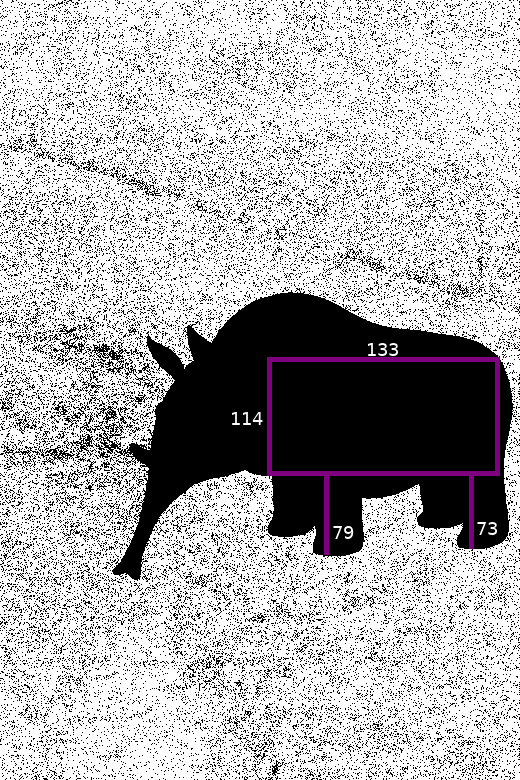
\includegraphics[width=0.7\textwidth]{SkizzeIdee4}
	\caption {2D-Abstraktion von Bsp. 4}
\end{figure}